\documentclass[11pt,letterpaper,oneside]{report}
\usepackage[T1]{fontenc}
\usepackage[utf8]{inputenc}
\usepackage[english]{babel}
\usepackage{lmodern}
\usepackage{microtype}
\usepackage[margin=0.86in,headheight=16pt]{geometry}
\usepackage[table,dvipsnames]{xcolor}
\usepackage{graphicx}
\usepackage{booktabs,tabularx,longtable,array}
\usepackage{enumitem}
\usepackage{titlesec}
\usepackage{fancyhdr}
\usepackage{hyperref}
\usepackage{xurl}
\Urlmuskip=0mu plus 1mu\relax
\usepackage{tcolorbox}
\usepackage{listings}
\usepackage{tikz}
\usetikzlibrary{arrows.meta,positioning,shapes.geometric,fit,calc}
\usepackage{needspace}
\usepackage{amssymb}
\definecolor{ink}{HTML}{14253A}
\definecolor{navy}{HTML}{17385D}
\definecolor{blue}{HTML}{20739A}
\definecolor{pale}{HTML}{ECF4F8}
\definecolor{green}{HTML}{1D6C5C}
\definecolor{softgreen}{HTML}{EEF8F4}
\definecolor{border}{HTML}{D4DFE7}
\definecolor{grey}{HTML}{506174}
\hypersetup{colorlinks=true,linkcolor=navy,urlcolor=blue,pdfauthor={Micro-Frontend Engineering Documentation Suite}}
\titleformat{\chapter}[display]{\normalfont\sffamily\bfseries\color{ink}}{\Large\color{blue}\MakeUppercase{\chaptername} \thechapter}{8pt}{\Huge}
\titlespacing*{\chapter}{0pt}{-10pt}{24pt}
\titleformat{\section}{\Large\sffamily\bfseries\color{navy}}{\thesection}{0.7em}{}
\titleformat{\subsection}{\large\sffamily\bfseries\color{navy}}{\thesubsection}{0.6em}{}
\setlist[itemize]{itemsep=3pt,topsep=5pt,leftmargin=1.6em}
\setlist[enumerate]{itemsep=4pt,topsep=5pt,leftmargin=1.8em}
\pagestyle{fancy}\fancyhf{}
\fancyhead[L]{\footnotesize\sffamily MICRO-FRONTEND ENGINEERING SUITE}
\fancyhead[R]{\footnotesize\sffamily\docshort}
\fancyfoot[L]{\footnotesize\color{grey}Engineering edition | October 2026}
\fancyfoot[R]{\footnotesize\thepage}
\renewcommand{\headrulewidth}{0.35pt}
\renewcommand{\arraystretch}{1.2}
\setlength{\emergencystretch}{2em}
\lstdefinestyle{eng}{basicstyle=\ttfamily\footnotesize,keywordstyle=\color{navy}\bfseries,commentstyle=\color{grey},stringstyle=\color{green},breaklines=true,breakatwhitespace=false,columns=fullflexible,keepspaces=true,showstringspaces=false,frame=single,rulecolor=\color{border},backgroundcolor=\color{pale},xleftmargin=5pt,xrightmargin=5pt,aboveskip=10pt,belowskip=10pt,captionpos=b}
\lstdefinelanguage{JavaScript}{morekeywords={const,let,var,require,return,async,await,import,export,default,function,try,catch,new,true,false,undefined,module},sensitive=true,morecomment=[l]//,morestring=[b]',morestring=[b]"}
\lstset{style=eng}
\newtcolorbox{sourcebox}{colback=pale,colframe=border,arc=2pt,boxrule=0.6pt,left=8pt,right=8pt,top=7pt,bottom=7pt}
\newtcolorbox{engineerbox}{colback=softgreen,colframe=green!45,arc=2pt,boxrule=0.6pt,left=8pt,right=8pt,top=7pt,bottom=7pt}
\newcommand{\based}[1]{\begin{sourcebox}\textbf{BOOK-GROUNDED CONCEPT}\\#1\end{sourcebox}}
\newcommand{\added}[1]{\begin{engineerbox}\textbf{ENGINEERING EXTENSION}\\#1\end{engineerbox}}
\newcommand{\term}[1]{\textbf{\color{navy}#1}}
\newcommand{\criterion}[1]{\textbf{Acceptance:} #1}
\newcommand{\book}{\emph{Building Micro-Frontends}, 2nd ed.}
\newcommand{\refs}{\chapter*{References and Provenance}\addcontentsline{toc}{chapter}{References and Provenance}
\begin{enumerate}[leftmargin=*]
\item \textbf{Primary source:} Luca Mezzalira, \emph{Building Micro-Frontends: Distributed Systems for the Frontend}, 2nd ed., O'Reilly Media, published November 2025 (copyright 2026), ISBN 978-1-098-17078-3. Chapter and printed-page references are included throughout. This suite paraphrases and synthesizes concepts; it does not reproduce the book.
\item \textbf{Engineering extension:} Webpack Module Federation reference: \url{https://webpack.js.org/plugins/module-federation-plugin}.
\item \textbf{Engineering extension:} Next.js multi-zones: \url{https://nextjs.org/docs/app/guides/multi-zones}. Details are version-sensitive and must be checked against the deployed framework version.
\item \textbf{Engineering extension:} OWASP Application Security Verification Standard 5.0: \url{https://owasp.org/www-project-application-security-verification-standard/}.
\item \textbf{Engineering extension:} GitHub Actions secure use reference: \url{https://docs.github.com/en/actions/reference/security/secure-use}.
\end{enumerate}}

\titleclass{\chapter}{straight}\titleformat{\chapter}[hang]{\huge\sffamily\bfseries\color{navy}}{\thechapter}{.7em}{}\titlespacing*{\chapter}{0pt}{24pt}{13pt}
\newcommand{\docshort}{LEARNING CURRICULUM}
\begin{document}
\begin{titlepage}\thispagestyle{empty}
\vspace*{1.1in}{\Huge\sffamily\bfseries\color{navy} Prerequisite-Based Learning Curriculum\par}
\vspace{18pt}{\Large\sffamily\color{blue} Competency graph, guided sequence, weekly milestones, and mastery assessments\par}
\vspace{27pt}\noindent\color{blue}\rule{0.75\textwidth}{1.4pt}
\vspace{23pt}\par{\large\sffamily A companion to Luca Mezzalira's \emph{Building Micro-Frontends}, Second Edition}\par
\vfill\noindent\textbf{Document series:} Micro-Frontend Software Architecture and Engineering\\
\textbf{Version:} 1.0 \quad \textbf{Prepared:} October 2026\\
\textbf{Production format:} pdfLaTeX-compatible standalone source\\
\textbf{Scope:} Original synthesis plus explicitly identified engineering extensions
\end{titlepage}
\pagenumbering{roman}\tableofcontents\clearpage\pagenumbering{arabic}

\chapter{Audience, Competencies, and Prerequisite Model}
\based{The primary reading follows the source's Chapter 1--14 order. This curriculum reorders practice based on skills prerequisites: web runtime knowledge precedes runtime federation, and trustworthy delivery precedes production migration.}
\section{Target audience}
Frontend developers, software architects, tech leads, platform and DevSecOps engineers, and AppSec reviewers. The curriculum can be completed as a 16-week team learning program or used selectively by experienced engineers.
\section{Entry competencies}
\begin{tabularx}{\linewidth}{p{.26\linewidth}X}\toprule Domain & Baseline expectation \\\midrule
Web fundamentals & HTTP, browser security model, DOM, accessibility basics\\
Languages and build & JavaScript/TypeScript, modules, package managers, webpack/bundlers\\
Architecture & Layering, cohesion/coupling, API and domain boundaries\\
Delivery & Git, basic CI, integration testing, production environments\\
Security & Session/auth basics, XSS/CSRF, dependency risk and secrets handling\\\bottomrule\end{tabularx}
\section{Competency prerequisite graph}
\begin{center}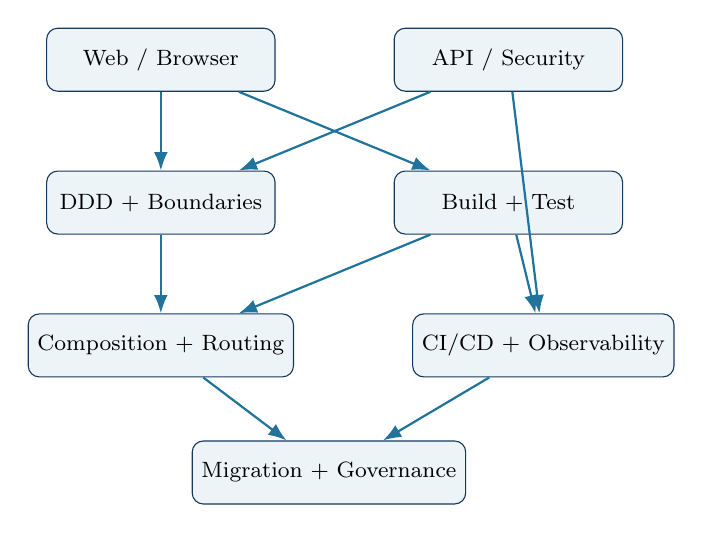
\begin{tikzpicture}[every node/.style={font=\footnotesize},n/.style={draw=navy,rounded corners,fill=pale,align=center,minimum width=2.9cm,minimum height=.8cm},a/.style={-{Latex},draw=blue,thick},node distance=10mm and 15mm]
\node[n] (web) {Web / Browser};\node[n,right=of web] (api) {API / Security};
\node[n,below=of web] (domain) {DDD + Boundaries};\node[n,right=of domain] (build) {Build + Test};
\node[n,below=of domain] (comp) {Composition + Routing};\node[n,right=of comp] (ops) {CI/CD + Observability};
\node[n,below right=8mm and -13mm of comp] (mig) {Migration + Governance};
\draw[a](web)--(domain);\draw[a](web)--(build);\draw[a](api)--(domain);\draw[a](api)--(ops);
\draw[a](domain)--(comp);\draw[a](build)--(comp);\draw[a](build)--(ops);\draw[a](comp)--(mig);\draw[a](ops)--(mig);
\end{tikzpicture}\end{center}
\chapter{Learning Outcomes by Level}
\begin{longtable}{p{.2\linewidth}p{.35\linewidth}p{.33\linewidth}}\toprule Level & Observable capability & Assessment \\\midrule
Foundation & Explain micro-frontends vs shared libraries; draw domain map & Written contrast + domain worksheet\\
Intermediate & Implement one vertical split; test remote failure & Runnable pilot + contract tests\\
Advanced & Choose SSR/client/hybrid; build secure pipelines and rollback & ADR + CI evidence + release drill\\
Expert & Set org-wide guardrails and measure success & Governance packet + capstone architecture review\\\bottomrule\end{longtable}
\chapter{Sixteen-Week Sequenced Plan}
\begin{longtable}{p{.09\linewidth}p{.28\linewidth}p{.2\linewidth}p{.33\linewidth}}\toprule Week & Subject & Reading chapters & Deliverable / checkpoint \\\midrule
1 & Web runtime, coupling, baseline & 1 & Baseline SPA and terms quiz\\
2 & Business capabilities and DDD & 1--2 & Capability map (Lab 1)\\
3 & Four decisions and review & 2 & Four provisional ADRs\\
4 & Vertical vs horizontal trade-offs & 3 & Weighted selection + sensitivity test\\
5 & Shell and route split & 3, 11 & Vertical pilot (Lab 3)\\
6 & Runtime federation & 4 & Remote contract and fallback (Lab 4)\\
7 & Web components and interfaces & 3--4, 10 & Isolation/compatibility (Lab 5)\\
8 & SSR, zones and caching & 5 & Zone experiment (Lab 6)\\
9 & API gateway/BFF/GraphQL selection & 9 & Auth-aware BFF (Lab 7)\\
10 & Contracts, anti-pattern repair & 10 & Compatibility suite (Lab 8)\\
11 & Automation strategies & 6, 8 & CI pipeline and evidence\\
12 & DevSecOps and supply chain & 6--8 & Security gates (Lab 9)\\
13 & Discovery, rollout, observability & 7 & Canary and rollback (Labs 10--11)\\
14 & Migration and case study & 11--12 & Three-wave migration decision\\
15 & Teams, governance, AI review & 13--14 & RFC/ADR review; AI validation record\\
16 & Integrative capstone & all & Architecture review and lab defense (Lab 12)\\\bottomrule\end{longtable}
\chapter{Assessment Design and Mastery Gates}
\section{Gate A: Conceptual readiness (after week 4)}
Define bounded context, vertical/horizontal split, and four decisions; compare a modular SPA to two distributed choices. \textbf{Pass:} at least 80\% on closed-note questions and no incorrect claim that remote JavaScript is isolated merely by federation.
\section{Gate B: Implementation readiness (after week 10)}
Demonstrate direct-route loading, independent build, explicit event/API contract, and isolated remote failure. \textbf{Pass:} all acceptance tests, including one failing negative-path test, reproduce from a clean checkout.
\section{Gate C: Production readiness (after week 13)}
Present security review, immutable artifact evidence, performance baseline, release attribution, and rollback. \textbf{Pass:} zero unresolved critical trust-boundary defects; release rollback drill completed and approved.
\section{Gate D: Architecture certification (week 16)}
Defend one chosen architecture under adversarial review. \textbf{Pass:} 80/100 on capstone rubric with explicit sign-off for security and recoverability. These percentages are locally defined learning policy, not a formal industry credential.
\chapter{Role-Specific Tracks}
\begin{tabularx}{\linewidth}{p{.22\linewidth}X}\toprule Role & Prioritized competencies and evidence \\\midrule
Frontend engineer & Weeks 1--10; accessible shell, runtime contracts, federation/SSR trade-offs\\
Staff architect & Weeks 2--5, 9, 14--16; bounded contexts, ADRs, selection framework and governance\\
Platform/DevOps & Weeks 8, 11--13; discovery, immutable delivery, SLO and operational runbook\\
AppSec engineer & Weeks 1, 6, 9, 11--13; trust boundaries, authorization, supply chain and negative tests\\
Engineering manager & Weeks 2--4, 14--16; ownership design, baseline metrics, investment decision\\\bottomrule\end{tabularx}
\chapter{Reinforcement and Reading Strategy}
\section{Spaced retrieval}
After each week's lab, create five short questions: two factual, one trade-off, one failure scenario, one organizational implication. Revisit at +1, +7, and +21 days, using fresh scenarios rather than memorized definitions.
\section{Case study discussion}
Use the book's fictional ACME case study (Chapter 12) to compare a vertical-first migration to an alternative horizontal split. Evaluate each under team topology, shell responsibilities, login, dependency sharing, design system, canaries, and recovery. Distinguish decisions shaped by ACME's context from universal engineering claims.
\section{AI-assisted learning guardrails}
\based{Chapter 14, pp. 369--397, treats AI as a development accelerator requiring engineering context, iteration, review, and refactoring, not as an autonomous source of architecture correctness.}
Provide AI with a domain map, contracts, operational constraints and quality gates; ask it to generate tests or alternative architectures; verify outputs through independent tests and human review. Do not upload credentials, private user data, or confidential architecture to tools without authorization.
\chapter{Capstone Portfolio and Evidence Matrix}
\begin{longtable}{p{.29\linewidth}p{.57\linewidth}}\toprule Artifact & Question it answers \\\midrule
Capability map and four ADRs & Why these domains, composition, routing, and communication?\\
Architecture scorecard & Why not a modular monolith or different composition?\\
Working pilot & Can teams build and release independently?\\
Contract and fault tests & What breaks under skew and partial outage?\\
Security checks & Are user and deployment trust boundaries controlled?\\
Performance and accessibility report & Is the composed user experience acceptable?\\
Release and rollback record & Can production recover quickly without rebuilding?\\
Migration plan and governance model & Can the system and organization sustain the change?\\\bottomrule\end{longtable}
\chapter{Program Completion and Next Steps}
Run a cross-functional design review with architecture, product, accessibility, platform, AppSec, and operations. Store capstone assets with reproducible tooling and an expiry/review date. A curriculum graduate should demonstrate not only how to implement a micro-frontend, but when \emph{not} to implement one.

\refs
\end{document}
